%\documentclass{cumcmthesis} 这里面是承诺书 
\documentclass[withoutpreface,bwprint]{cumcmthesis} 
\usepackage{ctex} % 支持中文
\usepackage{booktabs} % 支持三线表
\usepackage{geometry} % 支持页面布局
\usepackage[framemethod=TikZ]{mdframed}
\usepackage{url}   % 网页链接
\usepackage{subcaption} % 子标题
\usepackage{booktabs}
\usepackage{threeparttable}
\usepackage{svg}
\geometry{a4paper,scale=0.8} % 设置页面布局为A4纸,缩放比例为0.8

\title{基于XXX的XXX研究}
\tihao{C}
\baominghao{xxxx}
\schoolname{XMUM}
\membera{Liang Zimao}
\memberb{Wang Ziwen}
\memberc{Jiang Yecen}
\supervisor{  }
\yearinput{2024}
\monthinput{09}
\dayinput{08}

\begin{document}

\maketitle

\keywords{\textbf{0-1整数规划}\quad \textbf{动态规划} \quad \textbf{单边检验} \quad \textbf{概率统计分析}}

\section{摘要}
摘要内容

\section{问题重述}
\subsection{问题背景}
在当今的制造业环境中,由于市场对产品性价比要求的日趋严格,企业在保障产品功能及稳定性的同时,需要实现成本的有效管控,这意呈现出企业在采购、检测、组装及处置不合格产品等生产流程中需作出的明智决策。

产品成本的控制的保障始于生产过程的控制。在成本压力下,企业需在检测频率、成本
和产品质量间找到平衡点。尤其需要考虑到的是,不合格产品不仅会令公司损失产品本身的价值,还会影响品牌信誉和
客户满意度,增加售后服务成本。因此,企业的决策需综合考虑直接成本和潜在的市场
风险成本。数学建模为解决这一挑战提供了有力的工具,通过量化分析生产过程中的各种因
素,帮助企业在生产的流程决策中实现成本最优化

\subsection{问题重述}
问题一:供应商声称一批零配件的次品率不会超过某个标称值。需要设计一个抽样检测方案,以最少的检测次数确定是否接收这批零配件。假设标称值为10\%,需要针对两种情形给出具体结果:在95\%的信度下拒收次品率超过标称值的零配件;在90\%的信度下接收次品率不超过标称值的零配件。

问题二:结合已知两种零配件和成品的次品率,为生产过程的各个阶段制定决策方案以实现成本控制。决策包括是否检测零配件、是否检测成品、是否拆解不合格成品。

问题三:对包含多道工序和多个零配件的生产过程制定新的整体的生产策略,以实现成本控制。

问题四:假设问题2和问题3中的次品率数据是通过抽样检测方法得到的,重新评估和优化问题二、三生产过程中的决策。

\section{问题分析}
\subsection{问题一}
问题一是一个经典的概率统计问题。

问题要求设计一个抽样检测方案以确定是否接收供应商提供的零配件。核心在于如何在保证检测准确性的同时,尽可能减少检测次数。

在题意中供应商声称零配件的次品率不超过10\%,需要通过抽样检测来验证这一点。

首先,抽样检测的目标是评估零配件的实际次品率是否显著有别于(过高或者过低)供应商声称的10\%。为此,我们采用统计假设检验的方法,通过设定显著性水平(α),来决定在何种置信度下接收或拒收零配件。

考虑到对于是否接收这份零配件这个问题来说,我们只关注实际次品率是否会显著高于生成标称值(显著过高依然会选择接收),我们计划使用单侧检验,以减少所需的样本量。单侧检验中,设定零假设 $H_0: p \leq 0.1 $(次品率不超过10\%)和备择假设 $H_1: p > 0.1$ (次品率超过10\%)。通过计算p-value,我们可以在给定的置信度下判断是否拒绝零假设。

为提高检测效率,考虑使用正态分布逼近二项分布的方法。在样本量较大时,次品率的估计值可以近似为正态分布,这允许我们通过计算置信区间来快速判断次品率是否超出阈值。

最后,利用贝叶斯方法结合$Beta$分布来更新对次品率的信念。

综上所述,我们将通过结合统计假设检验、正态分布逼近和贝叶斯方法,设计出一个既准确又经济的抽样检测方案。通过这种方法,我们可以在保证检测结果可靠性的同时,最小化检测次数,从而为企业节省成本。


\subsection{问题二}
问题二是对生产-包装流程的最优处理策略,旨在最小化企业生产总成本。本质是一个0-1整数规划问题,因此应首先确定决策变量,即是否对零配件1、零配件2和成品进行检测,以及是否对不合格成品进行拆解。这些决策变量将直接影响生产成本和利润。接下来根据题目提供的数据,构建目标函数。目标是最大化利润。由于在本问题中,所有可能性仅有 6 $\times 2^{4}$ =96种,因此出于简化问题的考虑采用穷举法来得出所有情况,并求出最优决策

\subsection{问题三}
问题三要求对一个更加复杂的生产-包装流程确定最优处理策略,由于决策点的增加,可能性的数量非常大,采用与问题二相同的穷举法并不是足够优秀的方法

本问题要求在给定的零配件、半成品和成品的次品率条件下,通过决策方案优化生产过程,以最小化成本并最大化利润。问题核心在于如何通过检测和拆解策略,以及对不合格品的处理,来控制生产成本和保证产品质量。首先,需要对每个零配件是否进行检测做出决策,这直接影响到半成品的质量;其次,对半成品和成品的检测决策将决定最终产品的质量与市场表现;最后,不合格成品的拆解与调换损失也是成本控制的重要方面。

在分析过程中,难点在于如何量化检测与不检测的成本效益,以及如何评估拆解策略对成本和资源循环的影响。模型的转换将基于以下步骤:首先,建立零配件、半成品和成品的质量控制模型,分析检测与不检测的成本差异;其次,构建成品市场表现模型,评估不同检测策略对利润的影响;最后,设计拆解与调换策略的成本效益分析模型,以优化整体决策方案。通过这些模型的建立和分析,可以为生产过程提供科学的决策依据。

\subsection{问题四}
问题四分析

\section{模型假设}
\begin{itemize}
    \item 市场需求无限大,生产出的成品可以被全部卖出。
\end{itemize}


\section{变量说明}
\begin{table}[htbp]
    \centering
    \begin{threeparttable}
    \caption{变量说明表}
    \begin{tabular}{ccc}
        \toprule
        符号 & 含义 & 单位 \\
        \midrule
        $c_{i1}$ & 零配件$i$的次品率 &    \\
        $c_{i2}$ & 零配件$i$的检测成本 & 元 \\
        $c_{i3}$ & 零配件$i$的购买单价 & 元 \\
        $a_1$ & 占位 & 占位 \\
        $a_1$ & 占位 & 占位 \\
        $a_1$ & 占位 & 占位 \\
        $a_1$ & 占位 & 占位 \\
        $a_1$ & 占位 & 占位 \\
        \bottomrule
    \end{tabular}
    \begin{tablenotes}
        \item 注:未列出的符号以及重复出现的符号以出现处为准
    \end{tablenotes}
    \end{threeparttable}
\end{table}

\section{模型建立与求解}
\subsection{问题一模型分析}
问题一是一个经典的统计抽样检验问题,需要设计一个抽样检测方案以确定是否接收供应商提供的零配件。供应商声称零配件的次品率不超过10\%,企业需要通过抽样检测来验证这一声称。抽样检测的目标是评估零配件的实际次品率是否显著有别于供应商声称的10\%。为此,采用统计假设检验的方法,通过设定显著性水平(α),来决定在何种置信度下接收或拒收零配件。

\subsubsection{单边检验}

首先,我们采用单侧检验,检验当前抽样结果是否满足条件。在单次采样中,只有合格与不合格两种结果,因此样本中的合格数\(X\)可以被视为服从参数为\(m\)和\(p\)的二项分布:

$$X \sim \text{Binomial}(m, p)$$

在根据单边检验得出在假设($H0$:合格率 $p\leq0.9$)和(备择假设$H1$​:合格率 $p>0.9$ )条件下求出p-value。

采用单边检验p-value来确定是否有足够的证据拒绝零假设。如果p-value小于$1-\alpha$,则在$\alpha$的置信度下拒绝$H_0$,即认为次品率超过标称值,从而拒收这批零配件。

\subsubsection{正态分布逼近}

考虑到单次检测的效率问题,我们引入正态分布逼近二项分布的方法。在样本量较大时($m > 30$),次品率的估计值$\hat{p}$可以近似为正态分布:

$$\hat{p} \sim N(p, \frac{p(1-p)}{m})$$

这允许我们通过计算置信区间来快速判断次品率是否超出阈值。在$\alpha$的置信度下,置信区间为:

$$n = \left(\frac{Z_{\alpha/2}}{E}\right)^2 p(1-p)$$

其中,$Z_{\alpha/2}$是标准正态分布下的临界值,$E$是可接受的误差范围。

\subsubsection{贝叶斯方法}

最后,我们利用贝叶斯方法结合Beta分布来更新对次品率的信念。初始先验概率密度函数为$Beta(1,1)$,表明初始的次品率的可能性均匀分布在$(0,1)$上。随着检测的继续,对次品率的信念会发生改变,形成更准确的信念:

$$
P(A|B) = \frac{P(B|A)P(A)}{P(B)}
$$

其中,$P(A|B)$为后验概率,$P(B|A)$为似然函数,$P(A)$为先验概率,$P(B)$为边缘概率。更新的后验分布满足:

$$
A|B \sim Beta(1+k, 1+m-k)
$$

其中,$k$为$m$次检验中的次品数量

\subsection{问题一模型求解}
\subsubsection{单边检验}
样本中的合格数\(X\)被视为服从参数为\(m\)和\(p\)的二项分布:
$$X \sim \text{Binomial}(m, p)$$
假设$H0$:合格率 $p\leq0.9$
备择假设$H1$​:合格率 $p>0.9$
有
$$
p\text{-}value=\sum_{i=k}^{m}\binom{m}{i}0.9^i(1-0.9)^{m-i}
$$
其中$k$表示已经采样的合格的次数
如果$p\text{-}value$小于$1-\alpha$, 就可在$\alpha$的置信度下拒绝$H_0$, 这样就可以停止抽样得到所需置信度的结果
通过相同方法, 可以在$\alpha$的置信度下得出$p<0.9$的结论
\subsubsection{正态分布逼近(逼近二项分布)限制次数}
前面只使用单次检测有一个很严重的问题, 就是如果真实$p$ 的值极接近0.9(比如0.899)就会导致逐个抽样法中抽样次数需要极大才能出现显著性差异, 因此**引入正态分布逼近**的办法, 并且人为规定一个可允许的误差$E$, 来限制逐个抽样的次数
已知$X\sim Binomial(m,p)$ ,在较大的样本量下$(m>30)$, 可近似认为次品率估计值$\hat p$近似服从以下分布
$$
\hat p \sim N(p,{p(1-p) \over m})
$$
则有$\alpha$下的置信区间
$$
n=({Z_{\alpha \over 2} \over E})^2*p(1-p)
$$
$Z_{\alpha \over 2}$ 是标准正态分布下的临界值,$p$是检验标准(0.9)
- $\alpha=95\%,E=0.01$下$n\approx 3458$
- $\alpha=95\%,E=0.02$下$n\approx 865$
- $\alpha=90\%,E=0.01$下$n\approx 2435$
- $\alpha=90\%,E=0.02$下$n\approx 609$
*注: 这些检验次数n均大于30,说明确实可以使用正态分布逼近二项分布*
说明置信区间在90\%可允许的误差在2\%,在逐个采样法中单侧检验次数到达609后,若样本合格率没有显著高于0.9, 可以认为整体合格率小于0.9

\subsection{问题二模型建立}
问题二中,企业在生产过程中需要在多个阶段做出决策,包括是否对零配件进行检测、是否对成品进行检测,以及是否对不合格的成品进行拆解。以下是对这些决策的逻辑重构和详细分析:

成本效益模型
为了优化生产过程,企业需要最小化总成本,这可以通过成本效益分析模型来实现。总成本由以下几部分组成:
\begin{itemize}
    \item 装配成本:将零配件装配成完整成品所需的成本
    \item 检测成本:检测零配件或者成品所需的成本
    \item 拆解成本:对检验出不合格的成品进行拆解所需的成本
    \item 调换成本:调换进入市场的不合格成品的损失(包括隐形损失)
    \item 销售收益:卖出成品的收益
\end{itemize}

\subsubsection{装配的成本决策:}
企业需要装配成品,每装配一次,成本为:$C_{\text{单件装配}}$
由于企业装配

\subsubsection{零配件检测的成本决策:}
企业需要决定是否对零配件进行检测。如果选择检测,不合格的零配件将被丢弃;不检测则将直接用于装配。检测成本和不检测可能导致的损失:

检测成本:$C_{\text{检测}} = n \times C_{\text{单件检测}}$

不检测的损失(潜在) :$C_{\text{损失}} = n \times p_1 \times C_{\text{装配损失}} + C_{\text{调换损失}}$

如果检测成本低于不检测成本($C_{\text{检测}}<C_{\text{损失}}$),选择检测;反之则选择不检测。

\subsubsection{成品检测的成本决策:}
企业同样需要决定是否对成品进行检测,若不检测,则不合格的成品有可能进入

成品检测成本:$C_{\text{成品检测}} = m \times C_{\text{单件成品检测}}$

不检测的损失(潜在):$C_{\text{调换损失}} = m \times p_{\text{成品}} \times C_{\text{调换}}$

如果检测成本低于不检测成本($C_{\text{成品检测}}<C_{\text{调换}}$),选择检测;反之则选择不检测。

\subsubsection{不合格成品拆解的成本决策}
对于检测出的不合格成品,企业可以选择拆解以回收可用的零配件或直接丢弃。拆解成本和拆解收益之差是决策的关键:

拆解成本:$C_{\text{拆解}} = k \times C_{\text{单件拆解}}$ 

拆解收益:$C_{\text{拆解收益}} = k \times p_{\text{合格零件}} \times C_{\text{零件回收}}$

\subsubsection{综合决策模型}

综合考虑所有阶段的成本和收益,构建总成本模型,以确定是否进行检测或拆解,优化生产流程的成本结构
总成本

$$C_{\text{总}} = min(\sum (C_{\text{零件检测}} + C_{\text{装配}} + C_{\text{成品检测}} + C_{\text{拆解}}))$$

\subsubsection{采购策略}
由于次品率是已知的,因此出于节约成本的考虑,企业会按照比例来对两种零配件进行采购。
$a_n = \frac{N}{(1-c_{11} \times (1 - x_1))}$
$b_n = \frac{N}{(1-c_{21} \times (1 - x_2))}$(缺乏计算)

\subsubsection{对不合格成品处理策略}
对不合格成品来说,存在三种情形:

在质量管理和生产流程中,对成品的检测是一个关键步骤,以确保最终产品的质量符合标准。针对不合格成品的处理,我们可以构建一个决策模型来优化检测和组装流程。以下是对不合格成品处理流程的数学建模描述:

\begin{itemize}
    \item $A_{\text{pass}} $:零配件一合格。
    \item $A_{\text{fail}} $:零配件一不合格。
    \item $B_{\text{pass}} $:零配件二合格。
    \item $B_{\text{fail}} $:零配件二不合格。
\end{itemize}

\begin{itemize}
    \item  检测成本 $ C_{\text{test}} $:对一个零配件进行检测的成本。
    \item 组装成本 $ C_{\text{assemble}} $:组装一个成品的成本。
    \item 更换成本 $C_{\text{replace}} $:更换一个不合格零配件的成本。 
\end{itemize}

在两个零配件都在组装成品前被检测过的前提下,被拆解的成品得到的两个零部件是一定合格的,因此在此情况下可以直接将被拆分出来的成品不检测直接组装成成品

在两个零配件中只有一个在组装成品前被检测的情况下(同一决策下只对同一个零配件进行检测),可以仅对单个零件进行检测,在检测后组装出成品。具体流程图如下:

\begin{figure}[htbp]
    \centering
    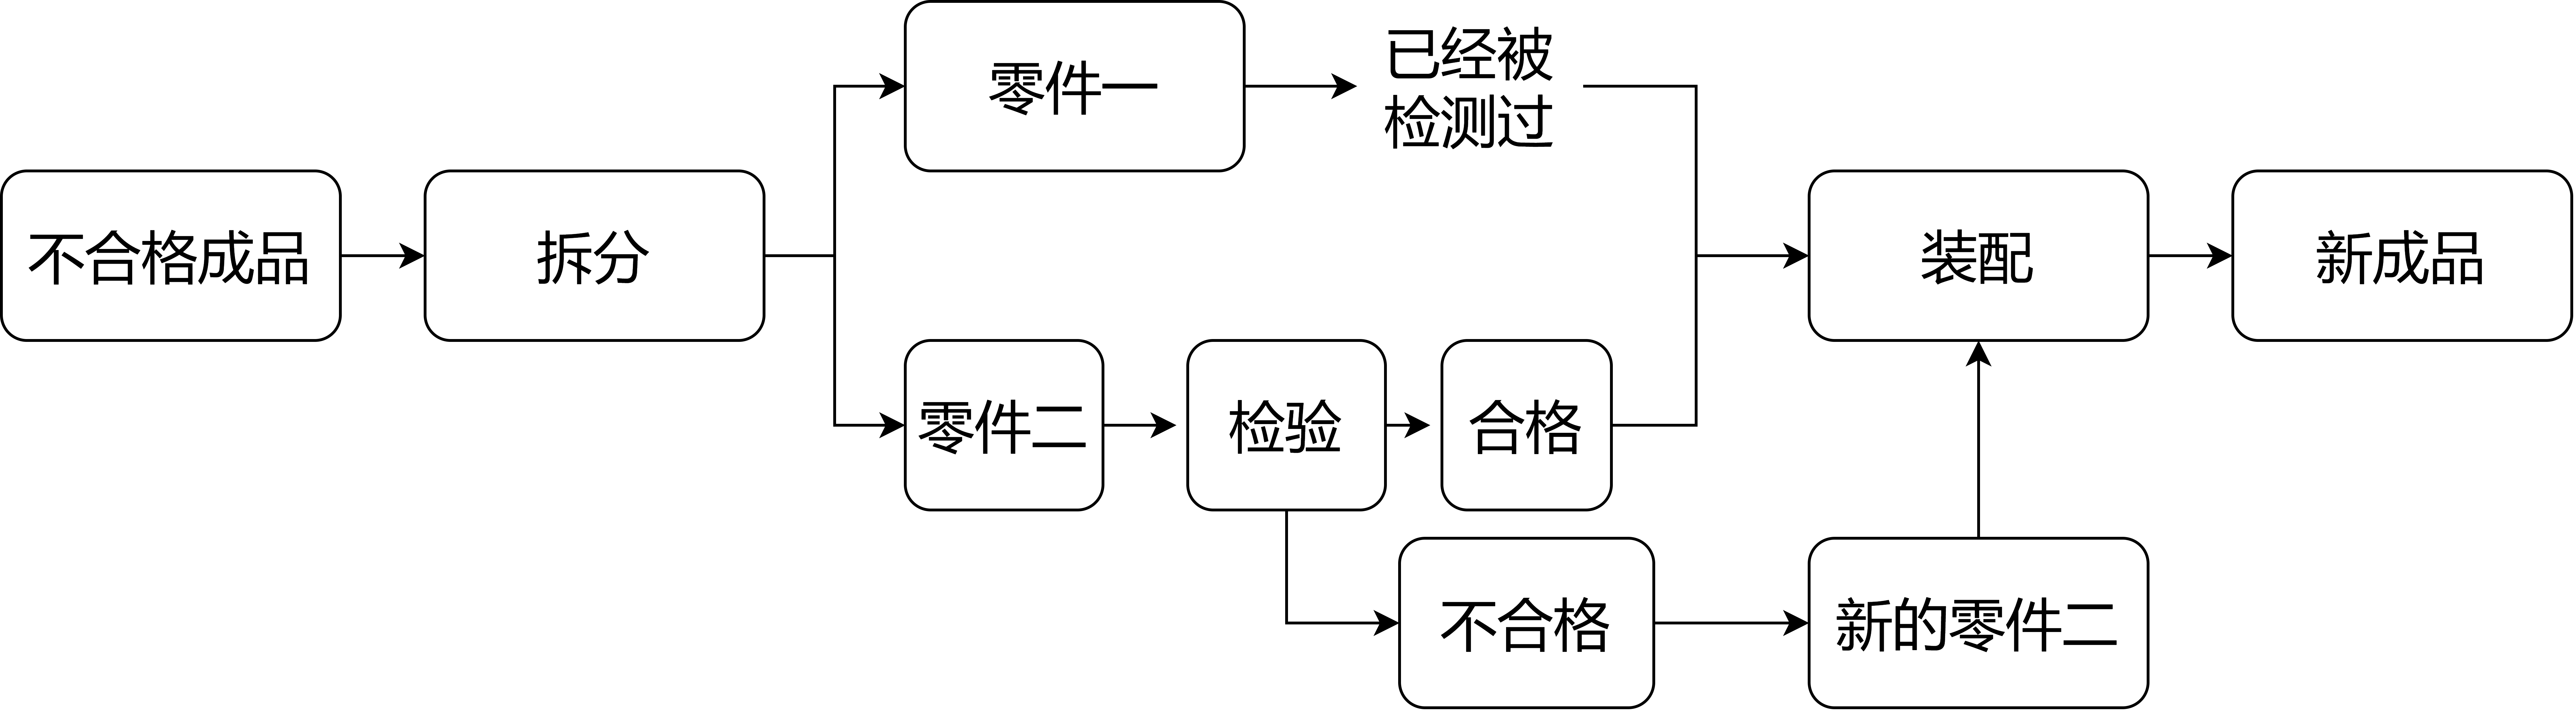
\includegraphics[width=0.6\textwidth]{figure/单零件检测流程.png}
    \caption{单零件检测流程}
    \label{2-checkout}
\end{figure}

在两个零配件在组装前都没有经过检测的情况下,被拆解的成品两个都进行检验,如果两个零配件都检验合格则直接组装,如果有不合格的零配件则直接替换且不对新的零配件不进行检测





\begin{itemize}
   \item 对于情形一,直接组装,成本为 $ C_{\text{assemble}} $。
   \item 对于情形二,成本为 $ C_{\text{test}} + C_{\text{assemble}} $ 或 $ C_{\text{replace}} + C_{\text{assemble}} $,取决于检测结果。
   \item 对于情形三,成本为 $ 2 \times C_{\text{test}} + C_{\text{assemble}} $ 或 $ C_{\text{test}} + C_{\text{replace}} + C_{\text{assemble}}$,取决于检测结果.
\end{itemize}

   

\subsection{问题二模型求解}
根据问题分析中提到的0-1整数规划-单目标优化的方法和模型建立中的建立思路,对模型的96中情况进行穷举,得到如下结果:
\begin{figure}[htbp]
    \centering
    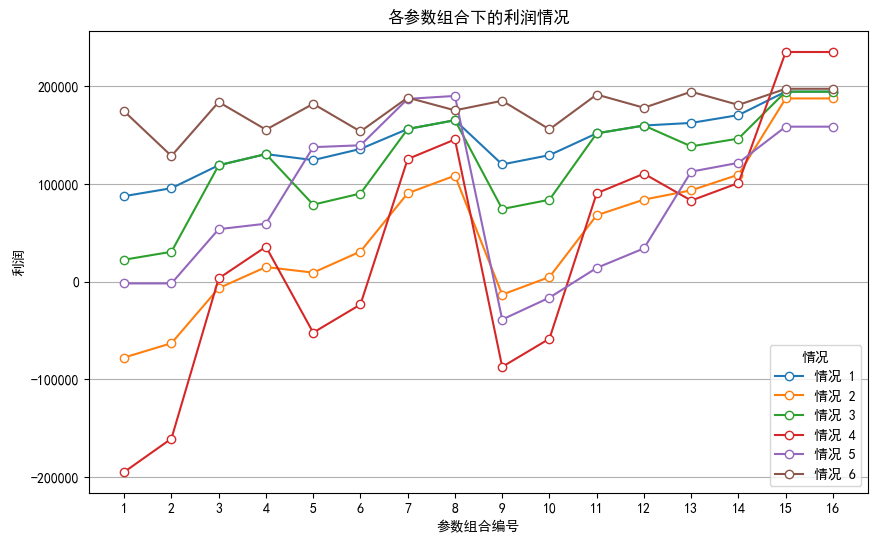
\includegraphics[width=1\textwidth]{figure/各参数组合的利润情况.png}
    \caption{各参数组合的利润情况}
    \label{2-profit}
\end{figure}

根据穷举得到的结果,我们可以知道在各类情况中,除了情况5的最优决策是8(1000,即检测零件一,零件一、成品都不检测)外,其他的所有情况最优决策策略都是15、16(1110、1111,即零件一、零件二、组装出的成品都进行检验)

\subsection{问题三模型建立}
问题三中,企业的生产流程大大的复杂化了,在问题三中的策略会更加复杂,决策点会大大增加,根据题意我们可以知道该问题有$ 2^{8} \times 8 \times 4 = 8192 $ 种不同的策略组合,策略量的大大提高使再次使用穷举法解决问题不再是一个足够优秀且有推广价值的数学建模解决方法


\subsection{问题三模型求解}

\subsection{问题四模型建立}

\subsection{问题四模型求解}


\section{模型分析与检验}
模型分析与检验内容。

\section{模型评价与改进}
模型评价与改进内容。

\section{参考文献}
参考文献内容。

\section{附录}
附录内容。

\end{document}

